\documentclass[11pt]{article}
\usepackage[T1]{fontenc}
\usepackage{lmodern}
\usepackage[margin=1in]{geometry}
\usepackage{amsmath,amssymb,booktabs,longtable,array,graphicx}
\usepackage{xurl}
\usepackage[colorlinks=true,linkcolor=blue,citecolor=blue,urlcolor=blue]{hyperref}
\usepackage{microtype}
\hypersetup{pdftitle={Strict Splitting Counts in Reconstructed Elliptic-Curve Candidate Streams},pdfauthor={Anonymous},pdfsubject={Exact reproduction and limitations},pdfkeywords={elliptic curves, Frobenius discriminant, reproducibility}}
\Urlmuskip=0mu plus 2mu
\setlength{\emergencystretch}{2em}
\newcommand{\F}{\mathbb F}
\newcommand{\artifact}[1]{\texttt{crypto:}\path{#1}}
\title{Strict Splitting Counts in Reconstructed Elliptic-Curve Candidate Streams:\\
An Exact Reproduction and Its Limits}
\author{Anonymous}
\date{29 October 2026}
\begin{document}
\maketitle
\begin{abstract}
We reproduce a previously reported arithmetic separation between published
elliptic curves and a particular set of unpublished candidates reconstructed
from historical seed streams. For each curve over a prime field, we count odd
primes at most 691 for which the Frobenius discriminant is a nonzero square.
All eleven unpublished candidates have larger counts than every publication
in their respective field, across four fields containing eight publications.
Two further publications, over the 384- and 521-bit fields, are retained without
unpublished same-field controls. Separate GMP and PARI implementations agree
on 6,342 odd-prime characters, 303 cutoff positions and all 4,480 label
assignments preserving publication counts within streams. Exactly 23
assignments separate at some cutoff in the declared family, reproducing the
prior report. Including zero characters destroys the separation at 691 in the
192-bit field. The cutoff, labels and reported outcome were known before this
replay: its contribution is computational reproduction, explicit convention
and cohort analysis, and an auditable evidence record. The result neither
authenticates a historical selection rule nor establishes a discrete-logarithm
advantage.
\end{abstract}
\noindent\textbf{Keywords:} elliptic curves; Frobenius discriminant; Elkies primes;
parameter generation; reproducibility; selection bias.

\section{Introduction}
The reconstruction of timestamp-initialized seed streams for historically
published NIST and ANSI elliptic curves leaves a separate question: why were
some other reconstructed candidates not published? Public accounts identify
an additional unexplained selection step after their stated arithmetic
screens \cite{anthropic,valsorda}. Recovering a seed stream and reconstructing
an eligible candidate do not, by themselves, show that the original program
visited that candidate or rejected it for a particular reason.

This paper examines an observation reported earlier by the account
asanso \cite{asanso}: at a small-prime cutoff of 691, published curves have
fewer strictly split primes than unpublished candidates in the same field.
We reproduce that observation on its fixed 21-choice cohort. We do not claim
discovery of the observation. The reported cutoff, outcomes and labels were
visible before the computational protocol was frozen.

Our contributions are an exact replay with a separate implementation,
a complete row-level account of the compared choices, reproduction of the
specified finite label calibration, and a sensitivity analysis separating
nonzero splitting from zero characters. We explain how this property relates
to generator/coefficient comparisons and identify the historical and
security conclusions that remain unsupported. No new point counting,
discrete-logarithm attack, runtime comparison or isogeny construction is
performed for this manuscript.

The paper is a replication note prepared from committed evidence
\cite{strictdata}. All displayed counts, indices, cutoffs and thresholds are
decimal. Parameter files retain their original explicit integer encodings.

\section{Arithmetic setting and precise statistic}
\subsection{Frobenius discriminant}
Let $E/\F_p$ be one of the nonsingular prime-field curves in the cohort.
The recorded full group order is $n=\#E(\F_p)$, including the identity;
the supplied cofactors are one. Set
\begin{equation}
 t=p+1-n,\qquad \Delta=t^2-4p.
 \label{eq:discriminant}
\end{equation}
For an odd prime $\ell\ne p$, let
$\chi_\ell(E)=(\Delta/\ell)\in\{-1,0,+1\}$ be the Legendre symbol.
The Frobenius characteristic polynomial modulo $\ell$ is
$X^2-tX+p$. A positive discriminant character gives two distinct roots and
two Frobenius-stable cyclic subgroup directions, hence two corresponding
degree-$\ell$ isogeny directions defined over $\F_p$.
This is standard point-counting structure
\cite{shparlinskiSutherland}. We compute the characters, not the isogeny maps.

Define the \emph{strict splitting count}
\begin{equation}
 S_L(E)=\#\{\ell:3\leq\ell\leq L,\ \ell\ {\rm prime},\
                                  \chi_\ell(E)=+1\}.
 \label{eq:strict}
\end{equation}
Separately record the zero-character and inclusive counts
\begin{equation}
 R_L(E)=\#\{\ell:3\leq\ell\leq L,\ \ell\ {\rm prime},\
               \chi_\ell(E)=0\},\qquad I_L(E)=S_L(E)+R_L(E).
 \label{eq:inclusive}
\end{equation}
The term \emph{Elkies prime} alone does not specify which count is meant:
definitions using a square discriminant can include zero. We use
Equation~\eqref{eq:strict} for the primary result and keep the inclusive
statistic separate. A zero character is not evidence that rational
isogenies are absent.

The prime 2 is excluded from these definitions. In the recorded cutoff
enumeration it is a zero-count boundary, with its character explicitly
unavailable under the odd-prime convention. Every cohort characteristic is
larger than the maximum cutoff 2,000, so no contributing prime equals $p$.

\subsection{Within-field separation}
Let $\mathcal P_f$ be the publications and $\mathcal U_f$ the compared
unpublished choices in field $f$. The fixed lower-count direction separates
at cutoff $L$ precisely when
\begin{equation}
 \max_{E\in\mathcal P_f}S_L(E)<\min_{E\in\mathcal U_f}S_L(E)
 \quad\text{for every field containing both labels}.
 \label{eq:separator}
\end{equation}
Thus each paired field has an upper threshold accepting every publication
and excluding every compared unpublished candidate. Ties prevent separation.
Thresholds follow the observed labeled envelopes; they are not authenticated
historical constants. Fields containing only publications remain in the
census but do not validate discrimination.

\section{Cohort, identities and historical scope}
The cohort contains ten publications and eleven unpublished reconstructed
candidates across six streams. The 192- and 239-bit streams each have three
publications; the 224- and 256-bit streams each have one publication with
unpublished controls. The 384- and 521-bit streams each supply one
publication without such controls. The 239-bit entries are ANSI examples;
we do not use P-239 as a NIST curve name.

A row key such as \texttt{p192-139} gives the field size and stream position.
It is a local record key, not a new standard name or an isomorphism claim.
The byte-preserved \path{data/inputs.tsv} fixes every row by stream, index,
exact $p,b,n$ and seed, with $a=-3\bmod p$. Historical publication names are
in Appendix~\ref{app:rows}. The original four supplied models have frozen
canonical ICV1 records in the earlier assessment identified by our data
manifest. No new active catalogue alias is introduced.

\paragraph{Ascertainment of the eleven.}
These eleven are a retrospective comparison set, not a proved complete
set of historical rejections. An earlier audit of the November 1997
X9.62 draft found 69 seed positions with certified full-prime-order
branches meeting its listed numerical conditions: ten published and
59 unpublished \cite{x962draft,acceptanceaudit}. The eleven form a subset
under additional root and order-width conventions. That broader result
is inherited evidence, not recomputed here; its full-prime-order census is
also only a lower bound on the draft's near-prime acceptance space.

The present separator therefore does not classify all 59 unpublished
positions, or every curve the original software might have examined.
No such extension was tested here. Historical use requires a justified
link between the actual implementation and this restricted cohort, or
independent predictions beyond it. We use \emph{unpublished} to describe
a recorded publication outcome, not observed visitation or rejection.

\paragraph{Conventions and missing data.}
The certified orders are inherited, not proved anew. The two P-224
coefficient representatives examined earlier preserve the same order
and hence this statistic. All eleven historical unpublished generators
remain unavailable. Assigned comparison points do not substitute for
historical observations.

\section{Reproduction method}
\subsection{Two implementations}
The native producer uses GMP integers, trial division for the small primes
and enumerated quadratic-residue tables. The separate verifier uses PARI
prime enumeration and Kronecker symbols. The producer enumerates bitmasks;
the verifier uses recursive label combinations and direct within-field
pair comparisons. Both reconstruct all six output files, including the
summary. Underlying GMP integer primitives may be shared; independence
here concerns the implementations, not independent integer libraries.

There are 302 odd primes through 2,000. Across 21 choices the programs
verify 6,342 odd-prime characters. They retain 303 prime cutoff positions,
including the exceptional boundary at 2. That boundary is not silently
converted to an ordinary character observation. Unavailable generators
and incomplete historical records are not numeric labels.

\subsection{Finite label calibration}
The enumeration preserves publication counts in each original stream:
\begin{equation}
 {5\choose3}{4\choose1}{8\choose3}{2\choose1}
 {1\choose1}{1\choose1}=4,480.
 \label{eq:labelspace}
\end{equation}
Every assignment receives the same 303 cutoffs and fixed lower-count
direction from Equation~\eqref{eq:separator}. Field thresholds follow
that assignment's publication envelope, as for the observed labels.
Singleton labels remain fixed. Strict and inclusive counts form separate
search families.

This is finite combinatorial calibration. A historical randomization-test
interpretation would also require exchangeability assumptions that are
not established. The enumeration accounts for the declared cutoff search,
not every trait, direction, coefficient convention or multivariate rule
explored elsewhere.

\subsection{Execution and refusal controls}
The protocol was frozen before the replay at source
\path{077c41e7d414cf72faf20bf9b474b7c35dae7bd8}, with digest
\begin{center}\small
\path{eeb7482bcda69477a360a7c28749b7f737d377dbe3298bec94346e4efbcdbbb7}.
\end{center}
This ordering protects the replay record; it does not make the externally
chosen hypothesis prospective.

Six phases were planned, attempted and completed in one actual attempt.
The positive control, producer and independent verifier each exited zero.
Deliberately corrupted character, calibration and summary outputs were
each refused with the required native exit one, identifying the intended
mismatching file. These are correct refusals, not successful verification
of corrupted data. Canonical export admission with file verification
reports zero findings.

Address space was limited uniformly to 1536 MiB. Watchdogs were 30 seconds
for the positive and each refusal control, and 120 seconds for production
and verification. These are resource limits, not measured scientific
runtimes. The uploaded checkpoint gate passed before execution. There
was no retry or restore of the actual scientific attempt. An earlier
planning invocation failed before any control ran because an external
timing utility was absent; the retained second invocation used shell
timing. The local exact-analysis fallback and cloud-tool limitations
are documented in the original record.

\section{Observed separation}
Table~\ref{tab:fields} reports exact values, not sample means with
sampling intervals. The upper envelopes are 60, 50, 57 and 57 for the
four paired fields. Every compared unpublished choice is above its
field's envelope. Figure~\ref{fig:counts} displays all 21 rows.

\begin{table}[htbp]
\centering\small
\begin{tabular}{@{}lrrl@{}}
\toprule
Field & Published $S_{691}$ & Unpublished $S_{691}$ & Upper bound\\
\midrule
192-bit & 57, 58, 60 & 61, 62 & 60\\
224-bit & 50 & 53, 56, 59 & 50\\
239-bit ANSI & 42, 57, 57 & 61, 63, 66, 67, 71 & 57\\
256-bit & 57 & 58 & 57\\
384-bit & 54 & no control & not tested\\
521-bit & 52 & no control & not tested\\
\bottomrule
\end{tabular}
\caption{Strict counts at decimal cutoff 691 and observed within-field
publication envelopes. Singleton publications do not validate a rule.
Source: native \texttt{data/at691.tsv}.}
\label{tab:fields}
\end{table}

\begin{figure}[htbp]
\centering
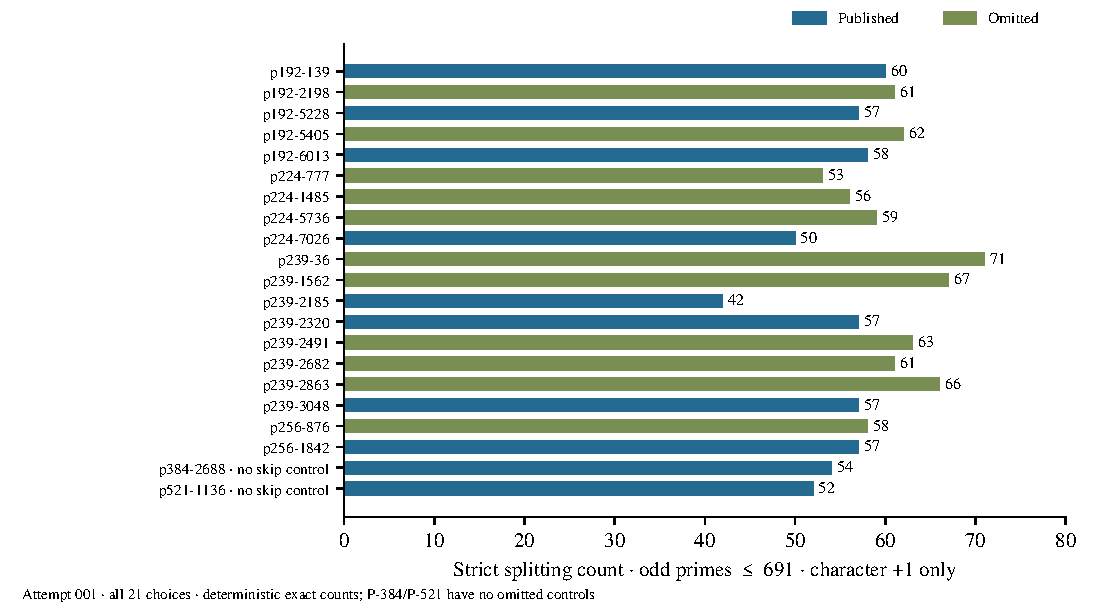
\includegraphics[width=\linewidth]{figures/strict-counts.pdf}
\caption{Every original choice, including singleton publications. This
vector rendering reuses the frozen recorded figure. Values are exact
$S_{691}$ counts, not attack costs or security scores.}
\label{fig:counts}
\end{figure}

A global threshold cannot fit these labels: published 192-bit count 60
exceeds unpublished 224-bit count 53. The 256-bit pair differs by one
count, an exact distinction rather than a demonstrated large security
effect. Across the complete cutoff family, the labels separate at exactly
691, 701, 709 and 769. These correlated cumulative counts are not
independent historical confirmations.

\subsection{P-192 and zero characters}
NIST P-192 is the publication at index 139. Its strict count is 60,
whereas unpublished indices 2198 and 5405 have counts 61 and 62.
The other publications have counts 57 and 58.
\begin{table}[htbp]
\centering\small
\begin{tabular}{@{}llrrr@{}}
\toprule
Index & Outcome & $S_{691}$ & $R_{691}$ & $I_{691}$\\
\midrule
139 & NIST P-192 & 60 & 3 & 63 \\
2198 & skipped & 61 & 0 & 61 \\
5228 & published & 57 & 1 & 58 \\
5405 & skipped & 62 & 0 & 62 \\
6013 & published & 58 & 1 & 59 \\
\bottomrule

\end{tabular}
\caption{The complete 192-bit subcohort. Zero characters change NIST
P-192 from 60 to 63 under inclusive counting.}
\label{tab:ramification}
\end{table}
P-192 has three zero-character primes, making its inclusive count 63.
The unpublished counts remain 61 and 62. An inclusive upper envelope
accepting every publication therefore also accepts those candidates:
the cutoff-691 separation fails. Zero characters cannot be interpreted
as absent isogenies or removed without specifying the convention.

\section{Calibration and inference}
Exactly 23 of the 4,480 permitted assignments have a separating cutoff
in the strict family, reproducing the prior report
\cite{asanso,strictdata}. At fixed cutoff 691, one assignment separates.
The smaller fixed-cutoff fraction is not a new confirmatory probability:
691 was selected retrospectively. Freezing a subsequent reproduction
does not remove the earlier selection.

The inclusive family has 20 successful assignments. This is a separate
sensitivity result, not a favorable replacement for the primary
calibration. Neither fraction adjusts for all earlier trait families or
the restriction to the eleven candidates. Neither is the probability
that selection was deliberate, that the pattern is a historical
coincidence, or that a trapdoor exists.

The counts are exact for this census. Uncertainty concerns cohort
ascertainment, historical label interpretation, unrecorded research
choices and external generalization. There is no untouched historical
holdout in this study.

\section{Generator and coefficient comparisons}
The strict statistic depends only on $p,n$. A different generator,
coordinate representation or $\F_p$-isomorphic model preserves them
and hence the profile. For a fixed field this is ultimately a property
of the point count, not a recovered formula for an unknown generator.

The earlier generator/coefficient census \cite{generatordata} checked
100,548 point-trait cells under repeated model and point controls,
and 147,875 same-field difference cells. Its 19,152 single-envelope
tests gave no complete separator; 880 public-scalar equality checks
gave no matches. These finite negatives do not exclude every
multivariate rule or generator relation. The eleven historical
unpublished generators remain unknown.

For $y^2=x^3-3x+b$, direct substitution gives
\begin{equation}
 x=0\Longrightarrow y^2=b,\qquad
 x=1\Longrightarrow y^2=b-2\pmod p.
\end{equation}
These defining-equation identities are not additional evidence of
hidden selection. Earlier conditional Lean proofs cover the
identities and seed-equation substitutions, with no authentication of
historical generator choices. The current census has native exact
verification, not a new Lean formalization. No new algebraic theorem
is asserted by this manuscript.

\section{Historical and security interpretation}
Frobenius splitting matters in point-counting algorithms
\cite{shparlinskiSutherland}, providing a mathematical reason to examine
this pattern in a generation setting. The count alone does not measure
an implementation's point-counting time, explain a preference for lower
counts or identify the original acceptance predicate. Earlier inclusive
counts and product-coverage experiments use different statistics and
retain their counterexamples.

A historical explanation needs an authenticated implementation or
decision trace fixing seed consumption, coefficient choices, actual
point-count inputs and keep/reject outcomes, or independently specified
predictions beyond this fitted cohort. The source audit
\cite{acceptanceaudit} and public accounts \cite{anthropic,valsorda}
supply no such trace. Reconstructed eligibility is not observed
visitation.

No discrete-logarithm algorithm follows from the separation.
An isogeny can transport a group problem without providing a cheaper
destination solver. An advantage requires explicit maps, subgroup
behavior, a destination algorithm and complete costs. Different point
counts also preclude interpreting the characters as isogeny maps
between the compared published and unpublished rows over the same
field. We construct no maps, recover no unknown scalars and provide
no curve-specific security certification. Neither weak publications
nor weak unpublished candidates are established.

\begin{figure}[htbp]
\centering
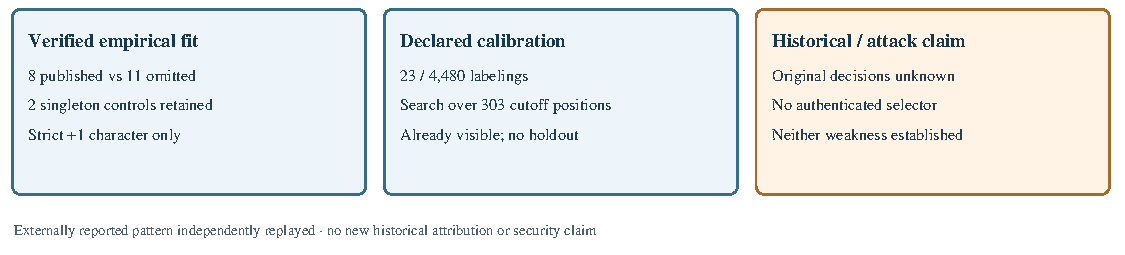
\includegraphics[width=\linewidth]{figures/evidence-boundary.pdf}
\caption{Evidence levels, reusing the frozen study's diagram. Exact
numerical conclusions do not supply the missing historical or attack
mechanism.}
\label{fig:boundary}
\end{figure}

\section{Reproducibility and data availability}
The package contains byte-preserved inputs, the 21-row table, native
summary and verification metadata, scientific source copies, editable
vector figures and LaTeX source.
\path{data/source-bindings.json} records source paths and digests.
The source snapshot is
\path{c51b0c32620ab43c73b1c0a34c236412f466f89a}; the actual execution
and preparation commits are separately fixed in the original protocol.

The full run archive is addressed by SHA-256
\begin{center}\small
\path{666660f97e6a7e2e9693a74789b39ae25e11a4baddbcae031d2fd02e3b7ac899}.
\end{center}
Its 96 regular members include native evidence and refusal controls.
The delivery record reports a full remote download and all-member
verification. Preparation/document archives, failed planning records,
binary bindings, protocol and limits remain preserved. Library
versions are pinned, not bundled. This manuscript adds no scientific
rerun, factorization or point-count certificate. Typesetting checks do
not constitute cryptographic replay.

The README explains PDF compilation, evidence bindings and access to
the original canonical export and complete raw record. The wider
arithmetic and generator evidence retains its original provenance
\cite{generatordata,factordata}; indeterminate historical-tool results
remain indeterminate.

\section{Conclusion}
The prior strict splitting-count separation reproduces exactly on its
fixed 21-choice cohort, with eight publications and eleven unpublished
candidates in paired fields. Separate implementations and deliberate
corruption controls support the finite result. Its dependence on
excluding zero characters is visible in P-192; its calibration covers
only a declared cutoff family. The historical choice mechanism and
both weakness hypotheses remain open. Independently specified testing
on a justified expanded cohort, or authenticated original decision
evidence, would discriminate further.

\paragraph{Draft and assistance statement.}
This anonymous replication manuscript was prepared with AI assistance
in drafting and document production from the cited computation records.
Human authorship, scientific review and final submission metadata
remain to be supplied. No IACR acceptance or peer-review status is claimed.

\appendix
\section{Every recorded choice at cutoff 691}\label{app:rows}
The table retains every choice, including both singleton publications.
Names are historical publication names; exact parameters and stream
identities are in \path{data/inputs.tsv}.
\begin{longtable}{@{}llrrr@{}}
\caption{All native observations. P denotes published; U denotes
unpublished. Source: \texttt{data/at691.tsv}.}\label{tab:allrows}\\
\toprule
Record / historical name & Label & $S_{691}$ & $R_{691}$ & $I_{691}$\\
\midrule\endfirsthead
\toprule
Record / historical name & Label & $S_{691}$ & $R_{691}$ & $I_{691}$\\
\midrule\endhead
\texttt{p192-139} / NIST P-192 & P & 60 & 3 & 63 \\
\texttt{p192-2198} & U & 61 & 0 & 61 \\
\texttt{p192-5228} / prime192v3 & P & 57 & 1 & 58 \\
\texttt{p192-5405} & U & 62 & 0 & 62 \\
\texttt{p192-6013} / prime192v2 & P & 58 & 1 & 59 \\
\texttt{p224-777} & U & 53 & 4 & 57 \\
\texttt{p224-1485} & U & 56 & 3 & 59 \\
\texttt{p224-5736} & U & 59 & 2 & 61 \\
\texttt{p224-7026} / NIST P-224 & P & 50 & 3 & 53 \\
\texttt{p239-36} & U & 71 & 2 & 73 \\
\texttt{p239-1562} & U & 67 & 3 & 70 \\
\texttt{p239-2185} / prime239v1 & P & 42 & 1 & 43 \\
\texttt{p239-2320} / prime239v2 & P & 57 & 2 & 59 \\
\texttt{p239-2491} & U & 63 & 2 & 65 \\
\texttt{p239-2682} & U & 61 & 4 & 65 \\
\texttt{p239-2863} & U & 66 & 1 & 67 \\
\texttt{p239-3048} / prime239v3 & P & 57 & 1 & 58 \\
\texttt{p256-876} & U & 58 & 2 & 60 \\
\texttt{p256-1842} / NIST P-256 & P & 57 & 2 & 59 \\
\texttt{p384-2688} / NIST P-384 & P & 54 & 0 & 54 \\
\texttt{p521-1136} / NIST P-521 & P & 52 & 1 & 53 \\
\bottomrule

\end{longtable}

\section{Evidence map}
Paths are relative to the cited repository snapshot.
\begin{itemize}
\item Statistic, exact inputs, sources, protocol and results:
\artifact{research/nist_skip_criterion_20261025/strict_elkies_20261029/}.
\item Generator/coefficient census:
\artifact{research/nist_skip_criterion_20261025/generator_b_execution_20261029/}.
\item Conditional identity proofs:
\artifact{research/nist_skip_criterion_20261025/generator_b_20261029/lean/CurveEquation.lean}.
\item Draft and expanded-cohort audits:
\artifact{research/nist_skip_criterion_20261025/source_check_20261027/sources/}.
\item Proved-factor follow-up:
\artifact{research/nist_skip_criterion_20261025/factor_followup_20261026/}.
\end{itemize}
The computational claims are finite observations with separate native
verification. The splitting interpretation is standard background
\cite{shparlinskiSutherland}; the generator identities have earlier
conditional Lean proofs. Historical intent, exhaustive coverage of
mathematical traits and any solver advantage have no supplied proof.
\bibliographystyle{plain}
\bibliography{refs}
\end{document}
